\chapter{\IfLanguageName{dutch}{Stand van zaken}{State of the art}}%
\label{ch:stand-van-zaken}

% Tip: Begin elk hoofdstuk met een paragraaf inleiding die beschrijft hoe
% dit hoofdstuk past binnen het geheel van de bachelorproef. Geef in het
% bijzonder aan wat de link is met het vorige en volgende hoofdstuk.

% Pas na deze inleidende paragraaf komt de eerste sectiehoofding.

% Dit hoofdstuk bevat je literatuurstudie. De inhoud gaat verder op de inleiding, maar zal het onderwerp van de bachelorproef *diepgaand* uitspitten. De bedoeling is dat de lezer na lezing van dit hoofdstuk helemaal op de hoogte is van de huidige stand van zaken (state-of-the-art) in het onderzoeksdomein. Iemand die niet vertrouwd is met het onderwerp, weet nu voldoende om de rest van het verhaal te kunnen volgen, zonder dat die er nog andere informatie moet over opzoeken \autocite{Pollefliet2011}.

% Je verwijst bij elke bewering die je doet, vakterm die je introduceert, enz.\ naar je bronnen. In \LaTeX{} kan dat met het commando \texttt{$\backslash${textcite\{\}}} of \texttt{$\backslash${autocite\{\}}}. Als argument van het commando geef je de ``sleutel'' van een ``record'' in een bibliografische databank in het Bib\LaTeX{}-formaat (een tekstbestand). Als je expliciet naar de auteur verwijst in de zin (narratieve referentie), gebruik je \texttt{$\backslash${}textcite\{\}}. Soms is de auteursnaam niet expliciet een onderdeel van de zin, dan gebruik je \texttt{$\backslash${}autocite\{\}} (referentie tussen haakjes). Dit gebruik je bv.~bij een citaat, of om in het bijschrift van een overgenomen afbeelding, broncode, tabel, enz. te verwijzen naar de bron. In de volgende paragraaf een voorbeeld van elk.

% \textcite{Knuth1998} schreef een van de standaardwerken over sorteer- en zoekalgoritmen. Experten zijn het erover eens dat cloud computing een interessante opportuniteit vormen, zowel voor gebruikers als voor dienstverleners op vlak van informatietechnologie~\autocite{Creeger2009}.

% Let er ook op: het \texttt{cite}-commando voor de punt, dus binnen de zin. Je verwijst meteen naar een bron in de eerste zin die erop gebaseerd is, dus niet pas op het einde van een paragraaf.

% \begin{figure}
%   \centering
%   
\includegraphics[width=0.8\textwidth]{grail.jpg}
%   \caption[Voorbeeld figuur.]{\label{fig:grail}Voorbeeld van invoegen van een figuur. Zorg altijd voor een uitgebreid bijschrift dat de figuur volledig beschrijft zonder in de tekst te moeten gaan zoeken. Vergeet ook je bronvermelding niet!}
% \end{figure}

% \begin{listing}
%   \begin{minted}{python}
%     import pandas as pd
%     import seaborn as sns

%     penguins = sns.load_dataset('penguins')
%     sns.relplot(data=penguins, x="flipper_length_mm", y="bill_length_mm", hue="species")
%   \end{minted}
%   \caption[Voorbeeld codefragment]{Voorbeeld van het invoegen van een codefragment.}
% \end{listing}

% \lipsum[7-20]

% \begin{table}
%   \centering
%   \begin{tabular}{lcr}
%     \toprule
%     \textbf{Kolom 1} & \textbf{Kolom 2} & \textbf{Kolom 3} \\
%     $\alpha$         & $\beta$          & $\gamma$         \\
%     \midrule
%     A                & 10.230           & a                \\
%     B                & 45.678           & b                \\
%     C                & 99.987           & c                \\
%     \bottomrule
%   \end{tabular}
%   \caption[Voorbeeld tabel]{\label{tab:example}Voorbeeld van een tabel.}
% \end{table}

Als modern IT bedrijf is het belangrijk om de veiligheid van de data te garanderen. 
Dit is de reden waarom het bedrijf heeft gekozen voor een Zero Trust netwerkarchitectuur. 
Deze studie onderzoekt de implementatie van een Zero Trust Netwerkarchitectuur en een least privileged access model binnen de hybride cloudomgeving van een softwarebedrijf gebruikmakend van het netskope platform.
Als eerste stap in dit onderzoek is het belangrijk om de huidige situatie van het bedrijf te analyseren. 
Dit omvat een overzicht van de huidige security-risico’s en tekortkomingen in de huidige perimeterbeveiliging.
Dit wordt gedaan door een analyse van de huidige infrastructuur en de security-risico’s die hiermee gepaard gaan. Interviews met de IT-afdeling zullen ook een rol spelen in het identificeren van de huidige tekortkomingen.

Zero Trust is een steeds belangrijker wordend model voor netwerkbeveiliging, vooral in omgevingen waar gevoelige data verwerkt wordt. 
Het model is gebaseerd op de stelling dat geen enkel apparaat, gebruiker of systeem automatisch te vertrouwen is, zelfs niet als deze zich binnen het netwerk bevinden.~\autocite{Netskope2020} 
De nadruk ligt op het continu verifiëren van gebruikersidentiteit, het beperken van toegang tot strikt noodzakelijke bronnen (least privileged access), en het monitoren van netwerkactiviteiten om verdachte handelingen snel te identificeren en aan te pakken.

Netskope, het platform dat het bedrijf heeft gekozen voor hun Zero Trust implementatie, definieert Zero Trust als een beveiligingsmodel waarbij niemand blind vertrouwd wordt binnen het netwerk of toegang krijgt tot resources, applicaties of data totdat ze gevalideerd zijn als legitieme gebruiker met een legitieme behoefte~\autocite{Netskope2020}. 
De Security Service Edge (SSE) architectuur van Netskope implementeert deze principes via een data-centrische aanpak gebaseerd op zes kernpijlers:

\begin{itemize}
  \item User \& Device: Authenticatie en autorisatie van gebruikers en apparaten
  \item Network \& Environment: Segmentatie en toegangscontrole op netwerkniveau
  \item Application \& Workload: Applicatie-specifieke toegangscontrole en monitoring
  \item Data: Databescherming en classificatie
  \item Visibility \& Analytics: Continue monitoring en gedragsanalyse
  \item Automation \& Orchestration: Geautomatiseerde response en integratie
\end{itemize}

Volgens Microsoft is de kern van het Zero Trust-model gebaseerd op drie belangrijke principes: altijd verifiëren, nooit vertrouwen; minimaal toegang verlenen; en schade beperken bij inbreuk. Dit houdt in dat de toegang tot systemen of data niet alleen wordt beperkt op basis van de locatie van de gebruiker of het apparaat, maar altijd afhangt van de identiteit, rol en andere specifieke toegangsbeperkingen~\autocite{Microsoft2024}. Netskope implementeert deze principes via een gelaagde aanpak met Policy Enforcement Points (PEPs) op drie niveaus:
\begin{figure}
  \centering
  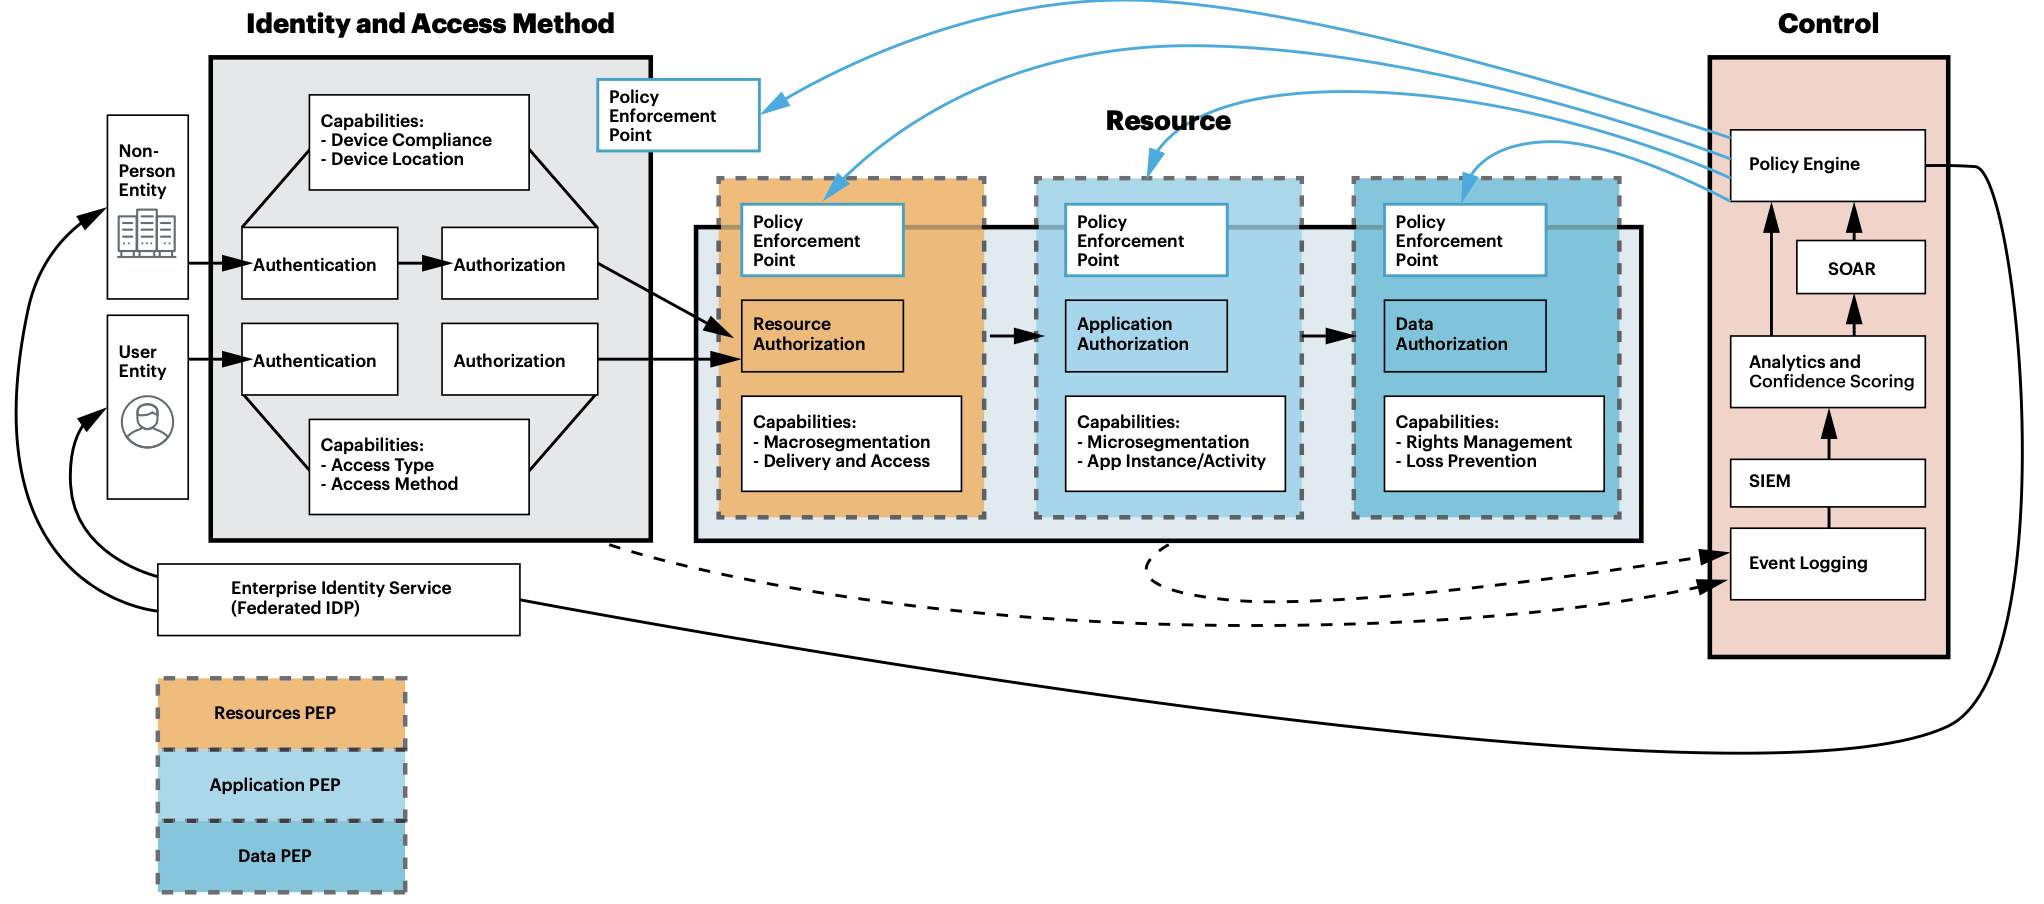
\includegraphics[width=1\textwidth]{Netskope-PEP.png}
  \caption[]{Policy Enforcement Points (PEPs) in Netskope's Zero Trust Security Service Edge (SSE) platform~\autocite{Netskope2020}}
\end{figure}

\begin{itemize}
  \item Network/Resource PEP: Controleert netwerktoegang en basiscommunicatie
  \item Application PEP: Beheert toegang tot specifieke applicaties en workloads
  \item Data PEP: Zorgt voor databescherming en compliance
\end{itemize}

Kaspersky benadrukt het belang van de technologieën die Zero Trust mogelijk maken, zoals multi-factor authenticatie (MFA), versleuteling van communicatie en geavanceerde netwerkmonitoringtools~\autocite{Kaspersky2024}. Netskope's platform integreert deze technologieën in een uitgebreid security framework dat onder andere bestaat uit:

\begin{itemize}
  \item Device en user authenticatie via een client certificaat infrastructuur
  \begin{figure}
    \centering
    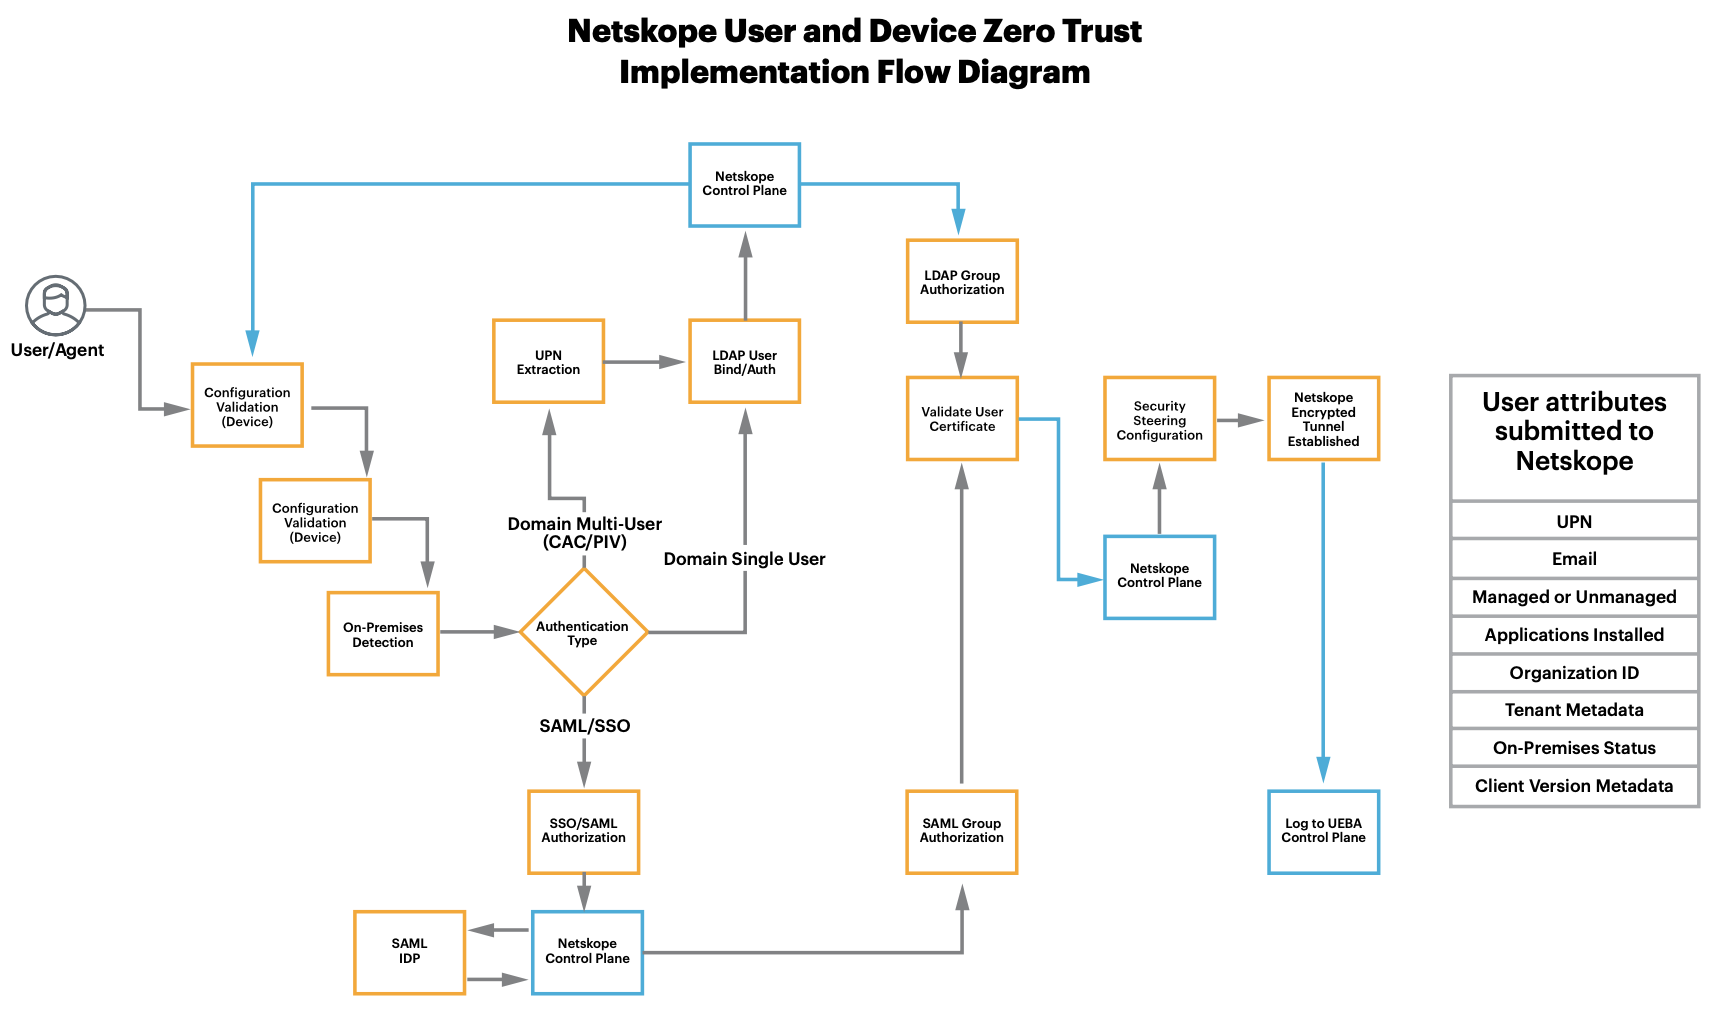
\includegraphics[width=1\textwidth]{Netskope-user-and-device.png}
    \caption[]{User \& Apparaat authenticatie in Netskope's Zero Trust Security Service Edge (SSE) platform~\autocite{Netskope2020}}
  \end{figure}

  \item Data Loss Prevention (DLP) met meer dan 3000 data identifiers en 1400 bestandstypes
  \begin{figure}
    \centering
    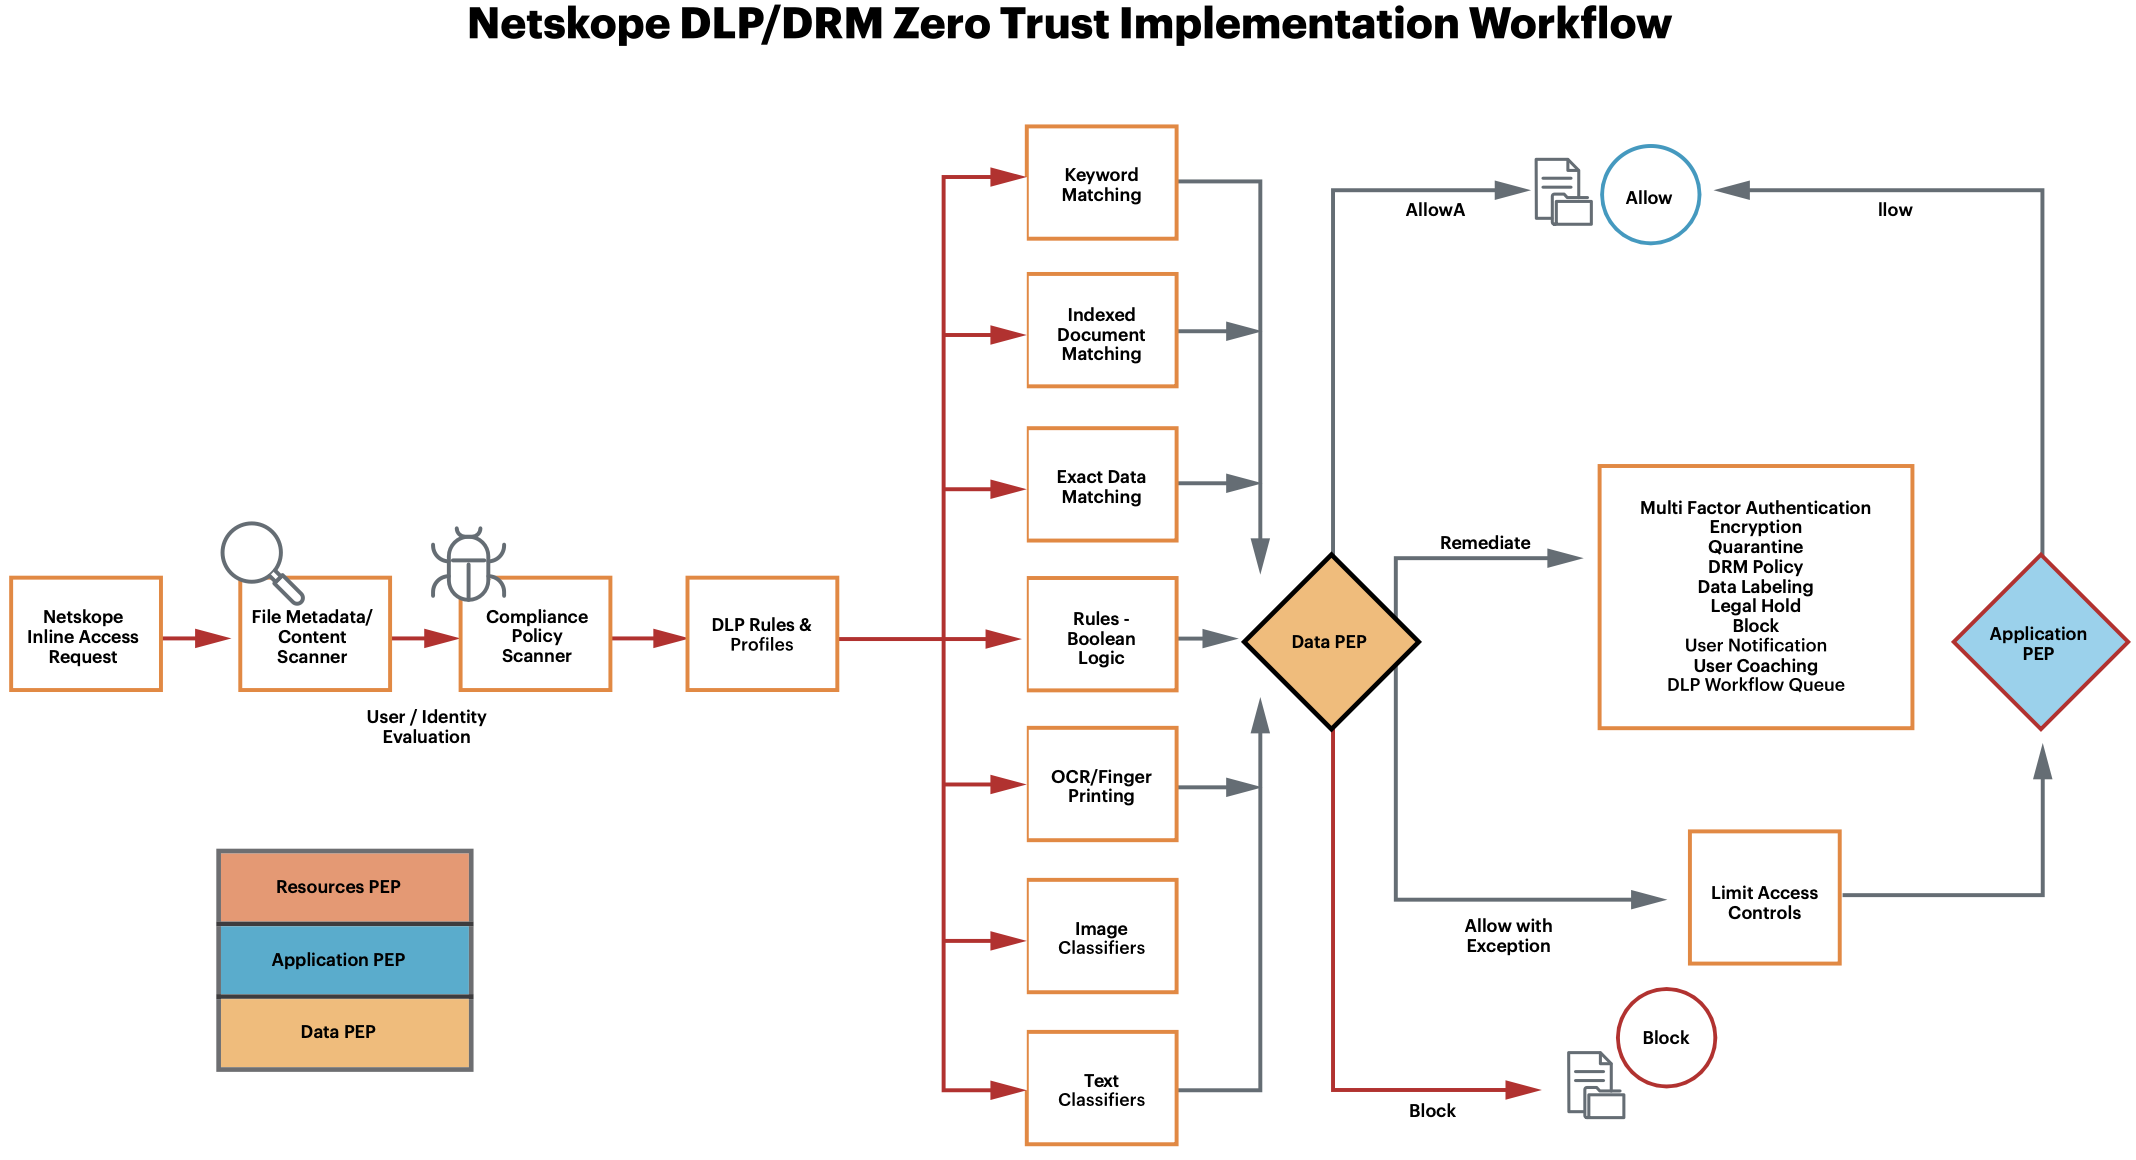
\includegraphics[width=1\textwidth]{Netskope-DLP.png}
    \caption[]{Data Loss Prevention (DLP) in Netskope's Zero Trust Security Service Edge (SSE) platform~\autocite{Netskope2020}}
  \end{figure}

  \item Software Defined WAN (SD-WAN) voor het samenvoegen van netwerken op site's met de cloud.
  \begin{figure}
    \centering
    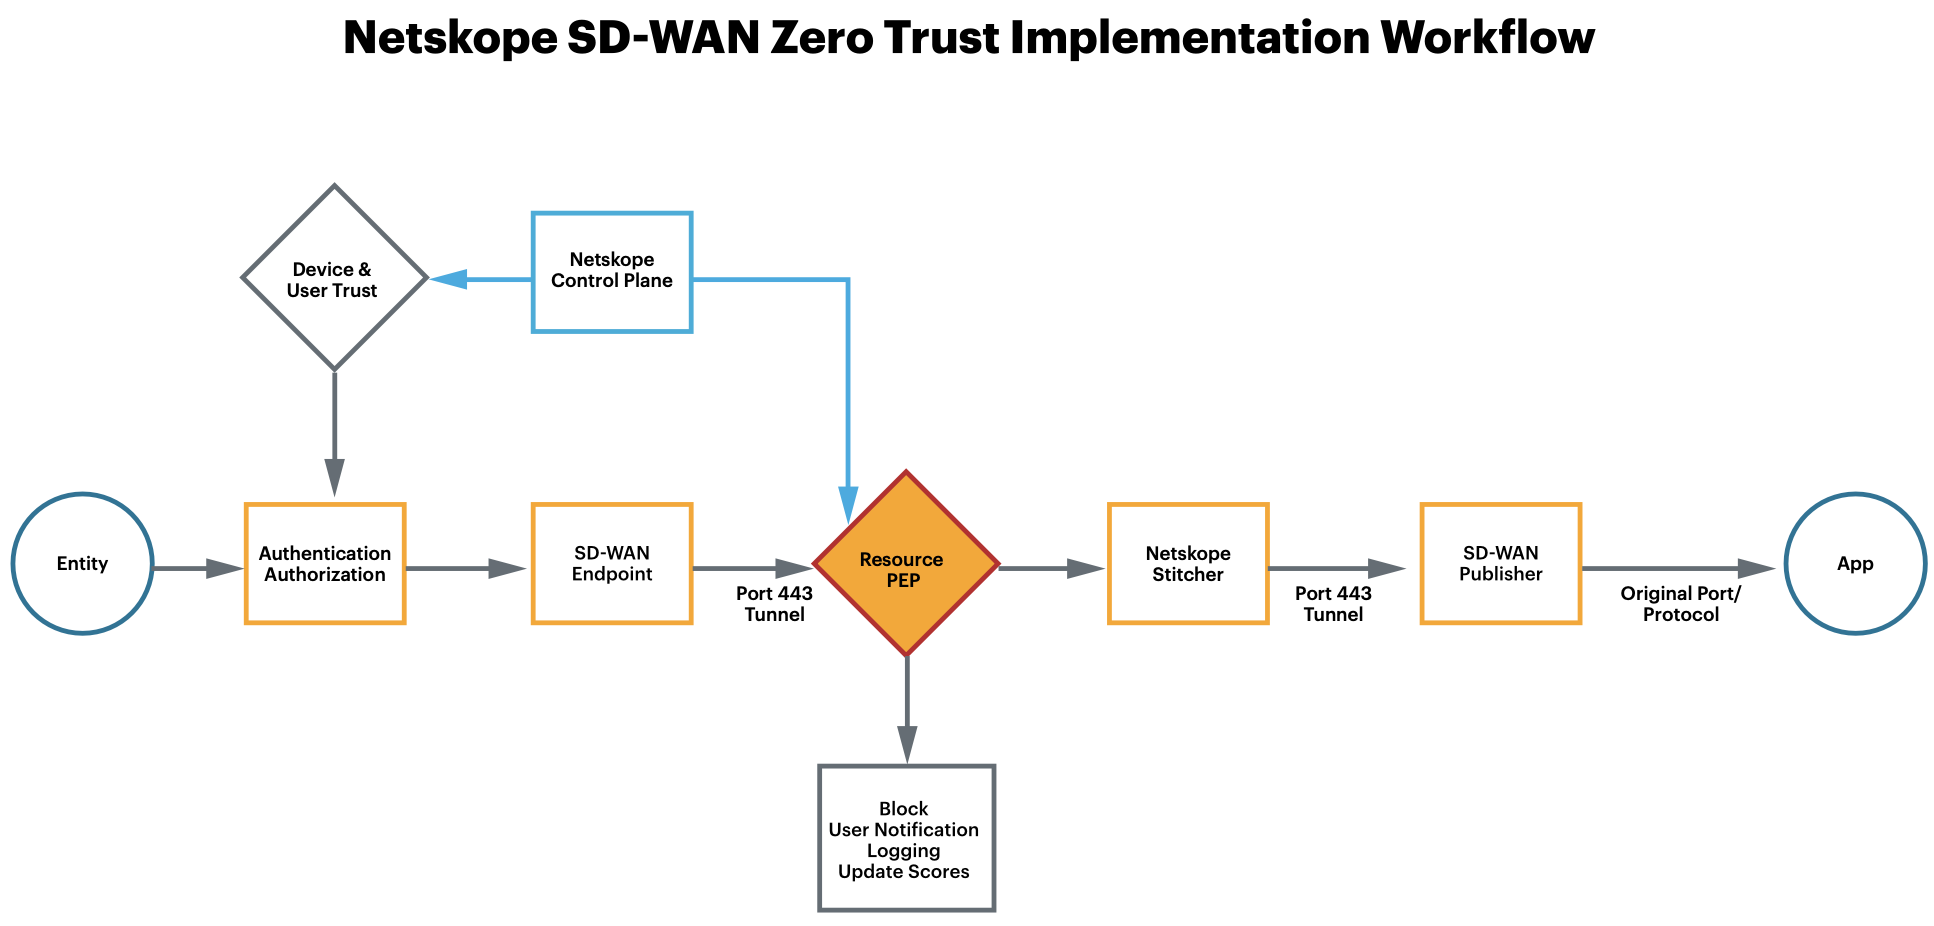
\includegraphics[width=1\textwidth]{Netskope-SD-WAN.png}
    \caption[]{Software Defined WAN (SD-WAN) in Netskope's Zero Trust Security Service Edge (SSE) platform~\autocite{Netskope2020}}
  \end{figure}

  \item Real-time threat protection met meer dan 40 threat intelligence feeds
\end{itemize}

De implementatie van Zero Trust vereist zorgvuldige planning, vooral in complexe netwerkomgevingen.

Uit onderzoek van MIT Lincoln Laboratory blijkt dat Zero Trust-architecturen bijzonder effectief zijn tegen insiderdreigingen, zoals misbruik van gecompromitteerde credentials of onbevoegde toegang door eigen medewerkers. 
Dit risico is relevant voor het onderzochte bedrijf, waar ontwikkelaars en externe partners toegang hebben tot gevoelige klantdata. 
MIT benadrukt dat een succesvolle Zero Trust-implementatie niet alleen technologische verandering vereist (zoals granular access control), maar ook organisatorische aanpassingen, zoals het trainen van medewerkers en het opstellen van een duidelijk beleid voor toegangsverificatie. 
Dit sluit aan bij Netskope’s focus op User \& Device workflows en gedragsanalyse, waarbij continue verificatie van gebruikers en apparaten centraal staat. 
Tegelijkertijd waarschuwt MIT voor de complexiteit van hybride implementaties, waarbij on-premises systemen en clouddiensten geïntegreerd moeten worden—een uitdaging die het bedrijf direct ondervindt en waar Netskope’s SSE-platform een antwoord op biedt.~\autocite{MIT2022}

Netskope biedt hiervoor een gestructureerde aanpak met specifieke operationele workflows:

\begin{itemize}
  \item User/Device workflow voor initiële authenticatie en continue validatie
  \item Network/Resource workflow voor toegangscontrole en segmentatie
  \item Data Protection workflow voor databescherming en compliance
\end{itemize}

Het onderzoek van Mutemwa et al~\autocite{ACM2021}. levert een belangrijke bijdrage aan ons begrip van de veranderende aard van cybersecurity in een post-pandemische wereld. Hun studie bevestigt dat traditionele perimeterbescherming fundamenteel is uitgedaagd door de verschuiving naar gedistribueerde werkomgevingen.
De auteurs concluderen dat organisaties moeten evolueren van een perimeter-gebaseerd beveiligingsmodel naar een meer complete benadering die rekening houdt met de realiteit van een uitgebreide, doorlatende bedrijfsgrens. Dit vereist een heroverweging van beveiligingsarchitecturen, met grotere nadruk op identiteitsbeheer, endpoint-beveiliging en gebruikerseducatie.
Deze studie onderstreept de noodzaak voor organisaties om hun cybersecurity-strategieën aan te passen aan een wereld waarin de traditionele grenzen tussen “binnen” en “buiten” het bedrijfsnetwerk steeds vager worden, een conclusie die aansluit bij de bredere verschuiving in de richting van zero-trust beveiligingsmodellen in de cybersecurity-gemeenschap.